\chapter{Evaluierung}

\section{Test}
Die Verifikation der DSL und ihrer Komponenten wird auf zwei Arten durchgeführt: Zum einen mit automatisierten Modultests und zum anderen mit manuellen Integrationstests. Erstere zielen darauf ab die Funktionsweise von Editor, Transformator und Validierer einzeln zu testen, um zu verifizieren dass diese ihre Anforderungen erfüllen. Letztere sollen das Zusammenspiel aller Module der DSL prüfen indem der Erstellungsprozess für verschiedene Konversationsroutings von der Modellierung bis zur Ausführung des Routings nachvollzogen wird.

\subsection{Automatisierte Tests}
Für die automatisierten Tests der DSL-Komponenten kommen Modultests, auch Unit Tests genannt, zum Einstaz. Befürworter der Unit Testing-Praktik befürworten an dieser Technik unter anderem eine hohe Testabdeckung und die frühe Detektierung von Fehlerzuständen [CITATION]. In der vorliegenden Ausarbeitung wird das Unit Test-Verfahren mit Hilfe des .NET-Test-Frameworks XUnit umgesetzt. Dabei werden Methoden mit einem Attribut als Test-Methoden designiert, welche dann von XUnit ausgeführt und ausgewertet werden. Die Testmethoden folgen dem Arrange-Act-Assert-Entwicklungsmuster. Hierbei ist eine Methode in drei Phasen aufgeteilt: In der Arrange-Phase werden die für den Test nötigen Vorbereitungen wir Objekt-Initialisierungen etc. durchgeführt. Anschließend folgt die Act-Phase, in der die zu testende Aktion durchgeführt wird. In der Assert-Phase wird das Testergebnis mit Assertions überprüft. Schlägt keine der Assertions fehl, gilt ein Testfall als bestanden.

\subsubsection{Editor}
In der Editor-Komponente werden zwei Klassen getestet: FlowDiagramViewModel und FlowDiagramControl. Die beiden Komponenten sind vor allem über die Datenbindung des Devexpress-Frameworks miteinander verbunden. Da das Testen dieser Verbindung jedoch außerhalb des Zuständigkeitsbereichs für die vorliegende Ausarbeitung ist, werden die beiden Klassen unabhängig voneinander getestet. Für FlowDiagramViewModel ist besonders das Verhalten bei Veränderungen in der Model-Schicht interessant, vor allem wenn es um das Hinzufügen oder Entfernen von Verbindungen geht. Folgende Aspekte der Klasse FlowDiagramViewModel werden unter anderem in den vorliegenden Unit Tests verfiziert: 

\begin{itemize}
\item Das Speichern von Flow-Instanzen im Dateisystem funktioniert
\item Das Laden von Flow-Instanzen aus dem Dateisystem funktioniert
\item Beim Hinzufügen von Connector-Instanzen werden die zugehörigen Input-Referenzen in betroffenen Outputs korrekt gesetzt
\item Beim Entfernen von Connector-Instanzen werden die zugehörigen Input-Referenzen in betroffenen Outputs auf null gesetzt
\item Beim Setzen einer Input-Referenz in einem Output wird eine entsprechende Connector-Instanz hinzugefügt
\item Beim Setzen einer Input-Referenz auf null in einem Output wird die entsprechende Connector-Instanz entfernt
\item Beim Verändern einer Input-Referenz in einem Output auf eine andere Input-Instanz wird der entsprechende Connector aktualisiert 
\end{itemize}

Auch bei der Klasse FlowDiagramControl fokussieren sich die Testfälle auf das Verhalten im Fall einer Veränderung der Daten, die per Datenbindung zur Verfügung stehen. Die Hauptaufgabe von FlowDiagramControl ist es, diese Daten auf Instanzen der Klasse FlowDiagramItem abzubilden. Da die eigentlich Darstellung der FlowDiagramItem-Instanzen von der Basisklasse und damit vom Devexpress-Framework überommen wird, wird dies nicht getestet. Stattdessen prüfen die Testfälle, ob es für jede Connector- und jede Node-Instanz eine entsprechende DiagramItem-Instanz gibt. Die Testfälle verifizieren daher folgende Anforderungen:

\begin{itemize}
\item Das Hinzufügen einer Node-Instanz fügt dem Diagramm eine entsprechende Flow\-Diagram\-Item-In\-stanz hinzu
\item Das Entfernen einer Node-Instanz entfernt auch die entsprechende Flow\-Diagram\-Item-In\-stanz
\item Das Hinzufügen einer FlowDiagramItem-Instanz fügt eine entsprechende Node-Instanz hinzu
\item Das Entfernen einer FlowDIagramItem-Instanz entfernt eine entsprechende Node-Instanz
\item Das Hinzufügen einer Connector-Instanz fügt dem Diagramm eine entsprechende Flow\-Dia\-gram\-Con\-nec\-tor-In\-stanz hinzu
\item Das Entfernen einer Connector-Instanz entfernt auch die entsprechende Flow\-Dia\-gram\-Con\-nec\-tor-In\-stanz
\item Das Hinzufügen einer FlowDiagramConnector-Instanz fügt auch eine entsprechende Connector-Instanz hinzu
\item Das Entfernen einer FlowDiagramConnector-Instanz entfernt auch die entsprechende Connector-Instanz
\item Das Ändern der Endpunkte einer FlowDiagramConnector-Instanz passt auch die entsprechende Connector-Instanz an
\end{itemize} 

\subsubsection{Transformator}  
TODO

\subsection{Manuelle Tests}
Bei den manuellen Tests geht es darum, das korrekte Zusammenwirken der einzelnen Komponenten zu testen. Daher werden alle Schritte, die für die Inbetriebnahme eines Konversationsroutings von Nöten sind, ausgeführt und die korrekte Funktionsweise anschließend verifiziert. Zu diesem Zweck werden folgende Schritte in der beschriebenen Reihenfolge ausgeführt:
\begin{description}
\item[Modellierung] \hfill \\
Hier wird mittels des Editors ein Modell angefertigt und abgespeichert. In dem Modell sind alle Arten von Instruktionen enthalten, welche auch alle mindestens einmal über einen Pfad des Konversationsroutings ausgeführt werden. Das Routing muss mindestens einen Zyklus in seinem Ablauf vorweisen. Zusätzlich sind mindestens je eine benutzerdefinierte Variable und Funktion im Routing enthalten, die auch in einer oder mehreren Script-Instruktionen verwendet werden. Bei der Modellierung des Routings müssen alle Editoren (Script-, Listen-, Ausdrucks- und Routing-Editor) mindestens einmal ausgeführt werden. Nach dem Editieren eines jeden Wertes muss durch erneutes Editieren überprüft werden, ob der Wert auch tatsächlich übernommen wurde. Treten während des Modellierens keine Fehler auf, wird das Routing im Dateisystem abgespeichert. 
\item[Ausführung] \hfill \\
Als nächstes wird die Routing Engine gestartet. Diese ist so konfiguriert, dass sie beim Start das im vorherigen Schritt modellierte Routing lädt und bei einem eingehenden Anruf ausführt.
\item[Anruf] \hfill \\
Nachdem die Routing Engine gestartet ist, kann das Modell über Anrufe getestet werden. Es werden so viele Anrufe getätigt, dass jeder Pfad des Routings einmal ausgeführt wurde und sich das Verhalten mit der Spezifikation des Modells deckt. Insbesondere wird stichprobenartig für jeden Pfad getestet, wie sich das System verhält wenn entweder der Anrufer oder ein beteiligter Agent frühzeitig den Anruf beendet. In diesen Fällen dürfen für ein Bestehen des Tests keine Anrufe auf Agenten- oder Kundenseite mehr übrig bleiben.
\end{description}
Ein Kandidat für ein Test-Routing mit dem die oben stehenden Schritte ausgeführt werden, ist in Abbildung \ref{fig:TestRouting} zu sehen. Neben dem Kriterium, alle Instruktionen zu beinhalten, bietet es eine überschaubare Anzahl an Pfaden die durch das Routing  führen. Dank der frühen DTMF-Instruktion kann zwischen drei Haupt-Pfaden gewählt werden. Werden die beiden Einstiegspunkte mit berechnet, genügen zur vollständigen  Abdeckung dieser Hauptpfade also acht Anrufe. Auf der Abbildung sind die Scripte sowie benutzerdefinierten Variablen und Funktionen, die zum Einsatz kommen, nicht zu sehen. Angelegt ist die Integer-Variable Count, welche im Set Variables-Knoten mit 0 initialisiert wird. Anschließend wird in der Branch-Instruktion abgefragt, ob Count größer als zehn ist und ob es sich um eine gerade Zahl handelt. Letzteres wird mit einer benutzerdefinierten Funktion IsEven überprüft. Die Branch-Instruktion nimmt also zu erst den False-Ausgang, welcher in das erste Script führt. Das Script dort inkrementiert diet Count-Variable um eins und führt zurück in die Branch-Instruktion. Diese Schleife wird solange ausgeführt, bis die Branch-Instruktion den True-Ausgang nimmt. Dieser führt das zweite Script aus, in der die benutzerdefinierte Funktion PrintTime aufgerufen wird, welche die aktuelle Systemzeit auf der Konsole ausgibt.

\begin{figure} %[hbtp]
	\centering
		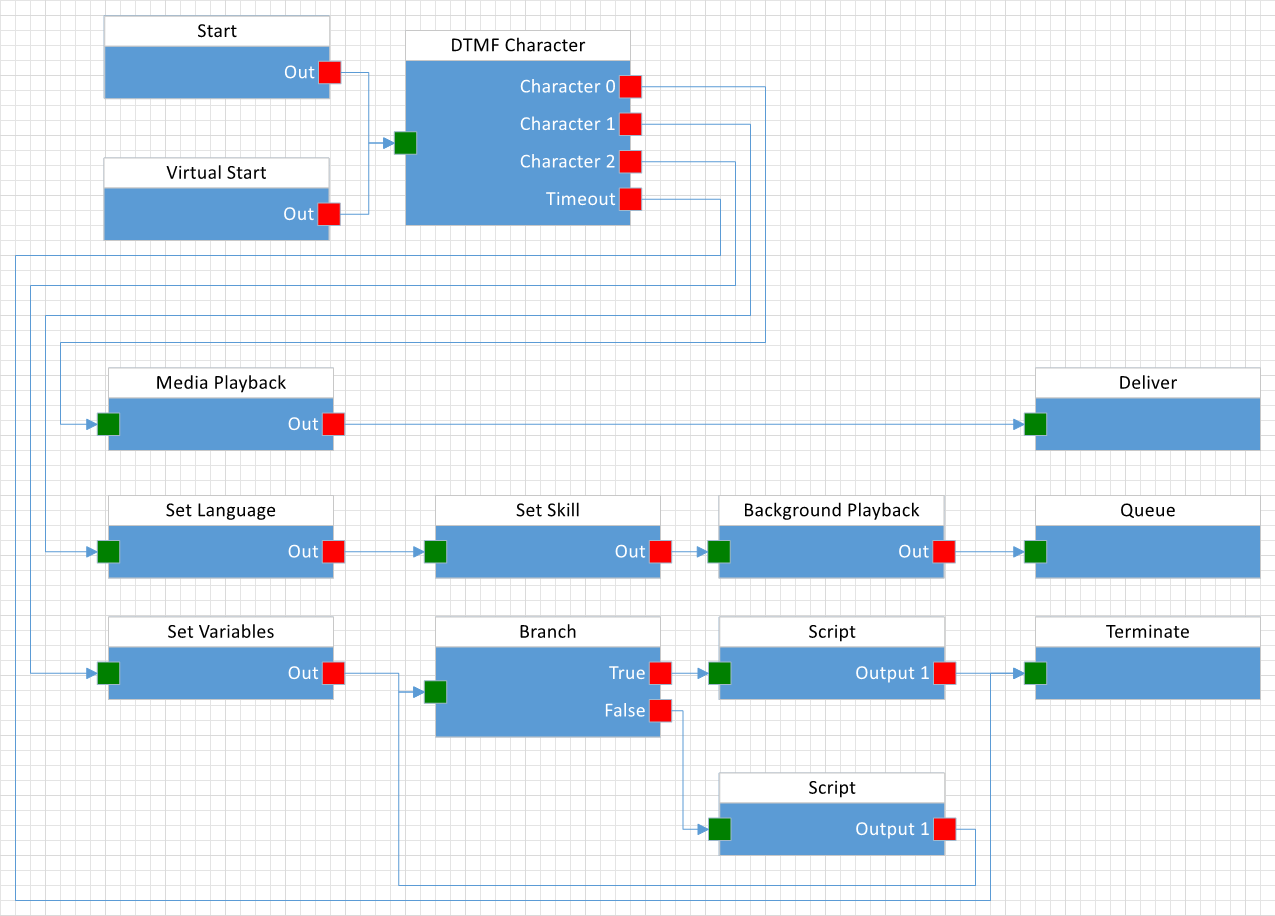
\includegraphics[width=\textwidth]{img/TestRouting.png}
	\caption[DSL-Modell für manuelle Tests]{Zu sehen ist das DSL-Modell, welches im Zuge von manuellen Tests zum Einsatz kommt.}
	\label{fig:TestRouting}
\end{figure}

\section{Metriken}
Bei der Umsetzung der DSL entstehen zwei Arten von Code. Die eine Art von Quellcode setzt das System um: Es handelt sich hierbei um den Quellcode, der den Editor und den Transformator implementiert. Die andere Art von Code ist der vom System generierte Code, also der CIL-Bytecode, der ein Routing implementiert. Beide Code-Sorten müssen eine hohe Qualität aufweisen, damit das System als Produkt zum einen einsatzfähig und zum anderen wartbar ist. Die im Folgenden beschriebenen Metriken vermessen und evaluieren diese beide Arten von Code. Berechnet wurden diese mit der Entwicklungsumgebung Visual Studio 2017 Ultimate. Zum Einsatz kommen hier die "Lines of Code", die zyklomatische Komplexität, auch als McCabe-Metrik bekannt, und der "Maintainability Index". Während die ersten beiden Metriken im Feld der Software-Architektur bekannt sind (unter anderem unter [CITATION] nachzulesen), ist der Maintainability Index ein Aggregat, welches verschiedene andere Werte in sich vereint. Es handelt sich um einen Ganzzahl-Wert von null bis 100, bei dem hohe Werte als positiv zu bewerten sind. Laut [CITATION 
\begin{comment}
https://blogs.msdn.microsoft.com/zainnab/2011/05/26/code-metrics-maintainability-index/ 
\end{comment}
] wird der Maintainability-Index folgendermaßen berechnet: 
\begin{dmath}
   \\max \left( 0, \left( 171 \\ - 5,2 * \log{\left(Halstead\ Volumen  \right)} \\ - 0,23 * \left( zyklomatische\ Komplexit\ddot{a}t \right) \\ - 16,2 * \log{\left(Lines\ of\ Code\right )} \\ \right) * 100 / 171 \right)
\end{dmath}
Das Halstead Volumen, beschrieben in [CITATION], ist ein weiteres Maß zur Einschätzung der Komplexität von Code. Code mit einem Maintainability Index zwischen 20 und 100 gilt als besonders wartbar. Ein Index unter 20 zeigt entweder eine mittelmäßige oder schlechte Wartbarkeit an. 

\subsection{Geschriebener Code}
In Tabelle \ref{tab:metrikenGeschriebenerCode} sind die gemessenen Metriken für den im Zuge der vorliegenden Arbeit händisch verfassten Code zu sehen.
\begin{center}
    \begin{tabular}{| l | l | l | l | l |}
    \hline
    Komponente & Namespace & LOC & zykl. Kompl. & Maint. Index\\ \hline
    Semantisches Modell & ConversationFlow.Core & 183 & 141 & 92 \\ \hline
    Editor & ConversationFlow.UI & 465 & 2818 & 78 \\ \hline
    Transformator & ConversationFlow.Generation & 730 & 299 & 76 \\ \hline
    Validator & ConversationFlow.Validation & 186 & 112 & 85 \\ \hline
    \end{tabular}
    \label{tab:metrikenGeschriebenerCode}
\end{center}
Das semantische Modell weist die niedrigste Komplexität auf. Dies ist nicht überraschend, da es sich um eine fast reine Datenstruktur handelt, die wenig programmatisches Verhalten aufweist. An zweiter Stelle kommt die Komponente der Modell-Validierung. Komplexe Strukturen, welche die Metriken negativ beeinflussen, konnten hier vermieden werden, da die meiste Arbeit, die solche Strukturen erfordert, an andere Komponenten ausgelagert wird. Eine deutlich höhere Komplexität weißt der Editor auf. Die Werte für diese Komponente lassen sich damit begründen, dass automatisch generierter Code des Devexpress-Framework in diesem Namespace enthalten ist. Devexpress benutzt einen sogenannten Component Designer, welcher "Boilerplate"-Code zum Erstellen von Windows Forms-Komponenten automatisch generiert. Dieser Code ist lang und dank seines Umfangs komplex. Zwar fallen die hohen Werte der Metriken dadurch auf, sind aber irrelevant, da der vom Component Designer generierte Code nicht von Hand lesbar oder editierbar sein soll und damit nicht die Komplexität des System widerspiegelt. Die laut dem Maintainability Index komplexeste Komponente ist der Transformator. 
\subsection{Generierter Code}
TODO

\section{Performanz}
TODO

\subsection{Geschriebener Code}
TODO

\subsection{Generierter Code}
TODO
